\section{Parameter estimation}

\subsection{Residue signal after reconstruction}\label{Nadya5}



\begin{figure}[!htbp]
\minipage{0.5\textwidth}%
\centering
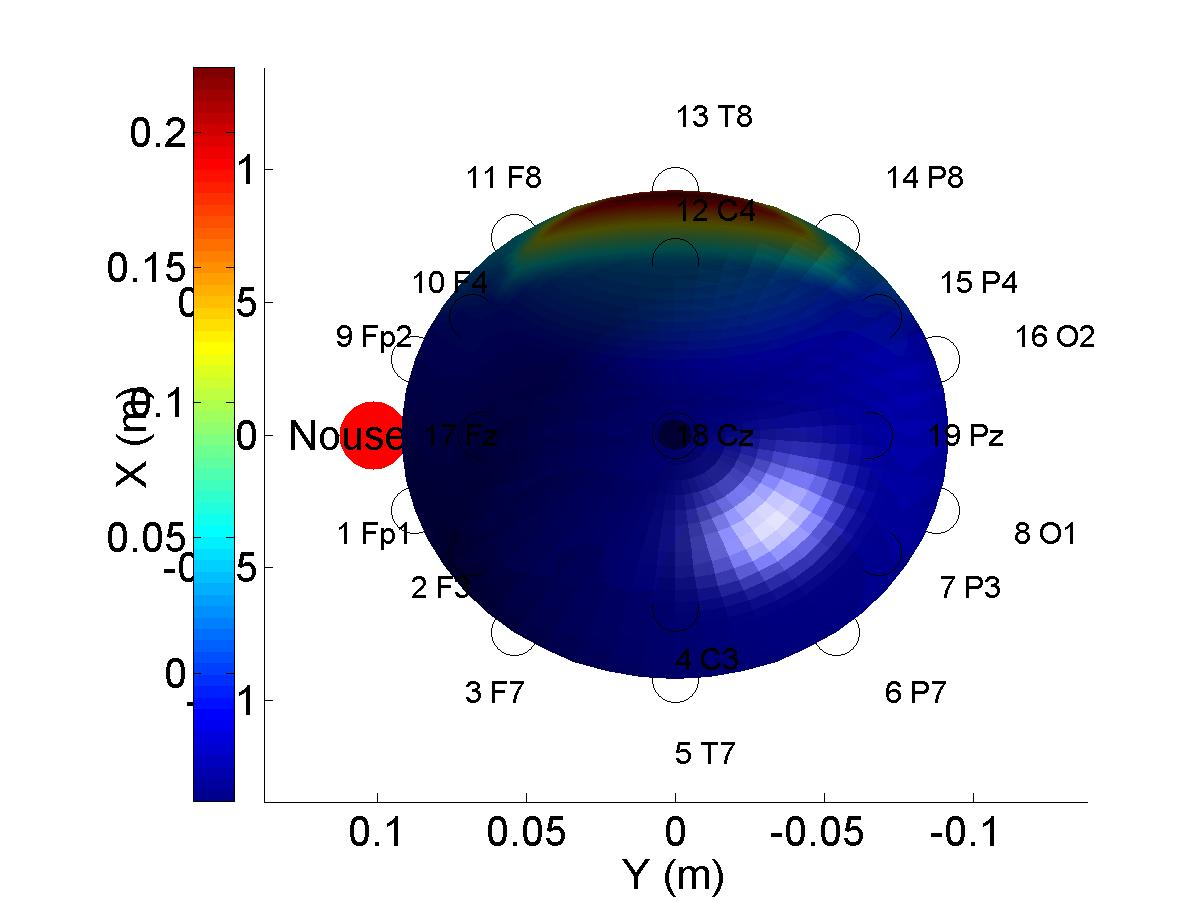
\includegraphics[width=1\textwidth]{103.jpg}\\
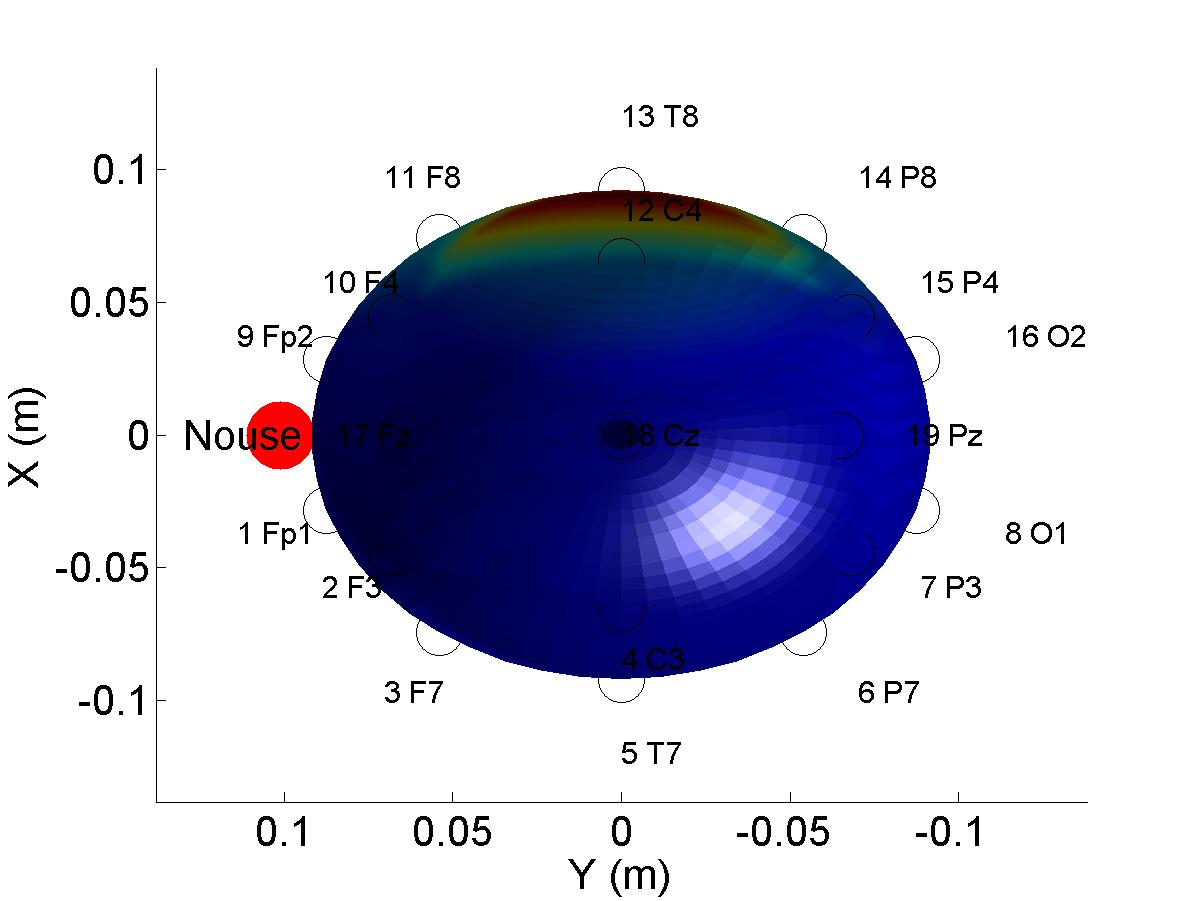
\includegraphics[width=1\textwidth]{105.jpg}\\
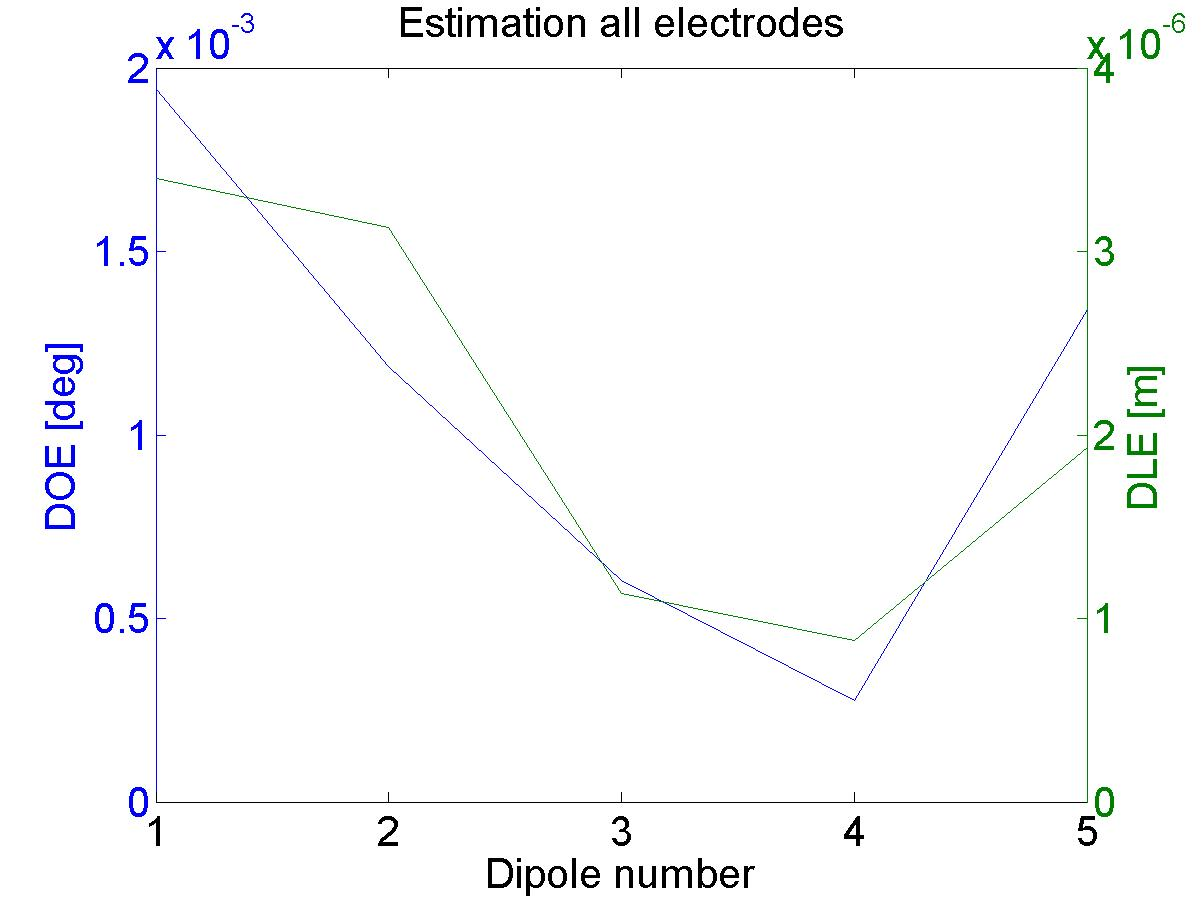
\includegraphics[width=1\textwidth]{107.jpg}\\
\subcaption{Filtered Signal}
\endminipage\hfill
\minipage{0.5\textwidth}%
\centering
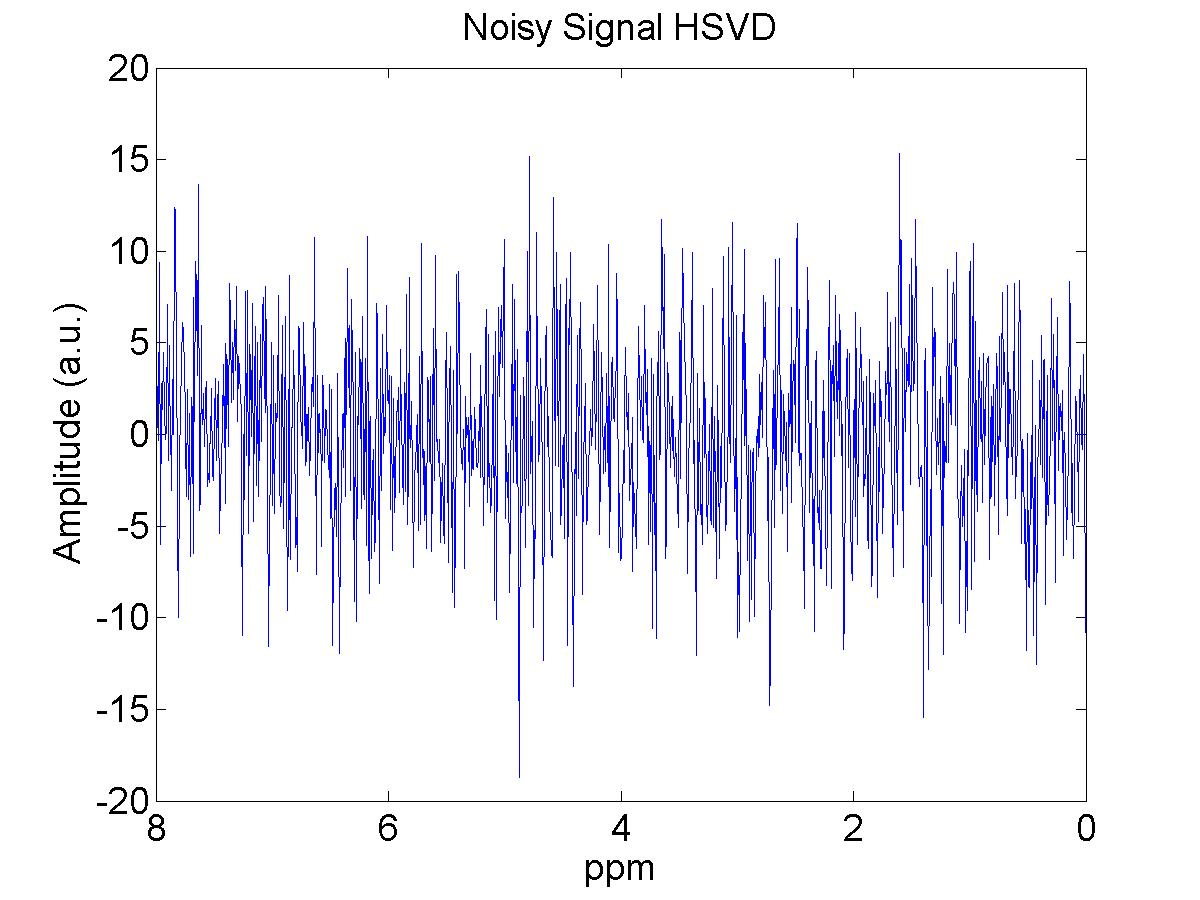
\includegraphics[width=1\textwidth]{109.jpg}\\
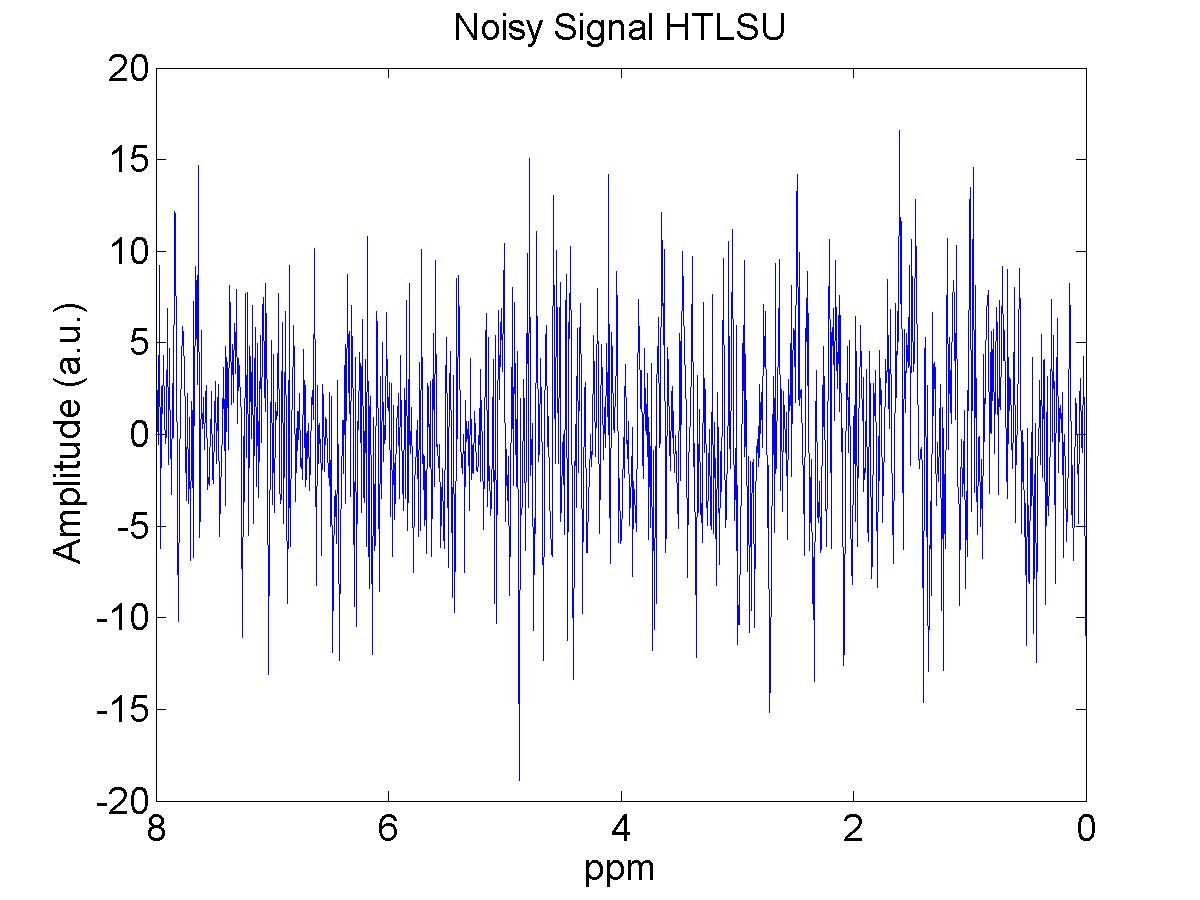
\includegraphics[width=1\textwidth]{111.jpg}\\
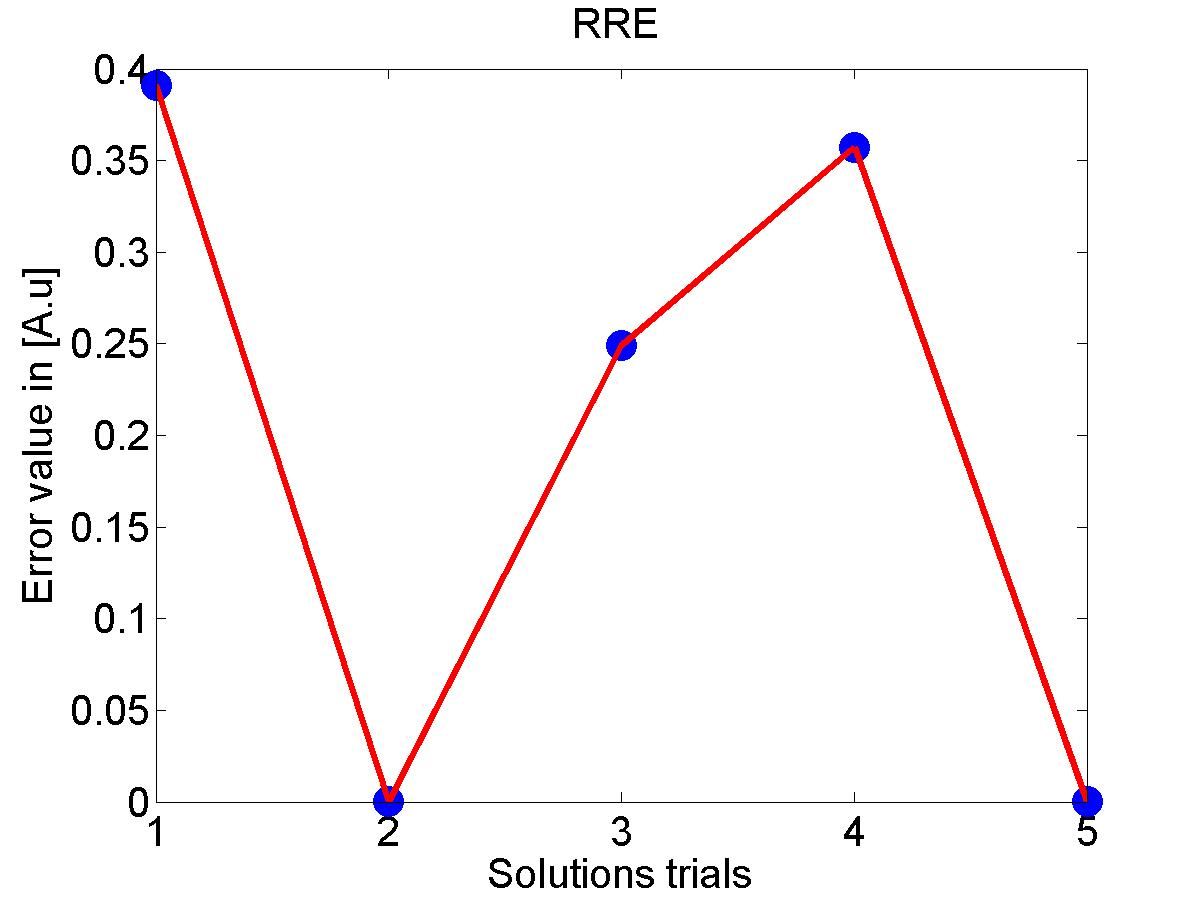
\includegraphics[width=1\textwidth]{113.jpg}\\
\subcaption{Noisy Signal}
\endminipage\hfill
\caption{Residue Signal}
\end{figure}

\newpage
\subsection{ Individual component for each method} \label{Nadya6}
\newcounter{themenumber}
\forloop[2]{themenumber}{102}{\value{themenumber} < 113}{

    %\arabic{themenumber}
    \begin{figure}[!htbp]
    \centering
    \includegraphics[width=1\textwidth]{\arabic{themenumber}.jpg}
    \caption{Individual component}
    \end{figure}
}



\newpage
\subsection{Parameter estimation}\label{Nadya7}

 \begin{table}[!htbp]
\centering
\caption{Frequency estimation \textbf{\textit{Hz}}}

\begin{tabular}{c c c c c c c c c c c c c c c c c c c c c c c c c c c c c c c } 
\hline 

\input{Textfiles/11.txt}  
\input{Textfiles/1.txt}  

\hline 
\end{tabular}
\end{table}





 \begin{table}[!htbp]
\centering
\caption{Damping estimation \textbf{\textit{Hz}}}

\begin{tabular}{c c c c c c c c c c c c c c c c c c c c c c c c c c c c c c c } 
\hline 
\input{Textfiles/11.txt} 
\input{Textfiles/2.txt}


\hline 
\end{tabular}
\end{table}





 \begin{table}[!htbp]
\centering
\caption{Amplitude estimation \textbf{\textit{a.u}}}

\begin{tabular}{c c c c c c c c c c c c c c c c c c c c c c c c c c c c c c c } 
\hline 

\input{Textfiles/11.txt} 
\input{Textfiles/3.txt}
\hline 
\end{tabular}
\end{table}



 \begin{table}[!htbp]
\centering
\caption{Phase estimation \textbf{\textit{Deg}}}

\begin{tabular}{c c c c c c c c c c c c c c c c c c c c c c c c c c c c c c c } 
\hline 
\input{Textfiles/11.txt}   
\input{Textfiles/4.txt}

\hline 
\end{tabular}
\end{table}  
    
    



\newpage

\subsection{Number of parameters}\label{A2}

Suppose we have the estimation model to be estimated with wgn\footnote{White Gaussian Noise} contamination:

\begin{equation}
x[n]=A_{0}+A_{1}n+wgn=\sum_{K=0}An^{k}+wgn
\end{equation}

We construct the Fisher information matrix in order to define the CR bound for $A_{1}$ and $A_{2}$.

\begin{equation}
    p(\hat{x};\hat{A})=\frac{1}{(2\pi\sigma^2)^{\frac{N}{2}}}exp\bigg\{-\frac{1}{2*\sigma^2}\sum_{n}(x[n]-\sum_{K=0}An^{k})^2\bigg\}
\end{equation}

\begin{equation}
    log(p(\hat{x};\hat{A}))=-\frac{N}{2}log(2\pi\sigma^2)-\bigg\{\frac{1}{2*\sigma^2}\sum_{n}(x[n]-\sum_{K=0}An^{k})^2\bigg\}
\end{equation}

\begin{equation}
   \frac{\delta log(p(\hat{x};\hat{A}))}{\delta \hat{A_{i}}} =\frac{1}{2\sigma^2}\sum_{n}2(x[n]-\sum An^{k})\frac{\delta \sum An}{A_{j}}=\frac{1}{\sigma^2}\sum_{n}(x[n]-\sum An^{k})n^{i}
\end{equation}

\begin{equation}
   \frac{\delta^2 log(p(\hat{x};\hat{A}))}{\delta \hat{A_{i}}\hat{A_{j}}} =\frac{1}{\sigma^2}\sum_{n}(n^{i}-\frac{\delta\sum An^{k}}{\delta A_{j}})=\frac{-1}{\sigma^2}\sum_{n}n^{i}n^{j}\Longrightarrow I(\hat{A})=I_{ij}=\frac{1}{\sigma^2}\sum_{n}n^{i}n^{j}
\end{equation}

Thereby it is concluded that information matrix $I(A_{0}A_{1})$ is :\\

$I = 
 \begin{pmatrix}
  \sum_n n^{0}n^{0} &  \sum_n n^{0}n^{01} \\
  \sum_n n^{1}n^{0} &  \sum_n n^{1}n^{1} 
 \end{pmatrix}
 = 
 \begin{pmatrix}
  N&  N(N+1)/2 \\
  N(N+1)/2 &  N(N+1)(2N+1)/6 
 \end{pmatrix}$


In case $\sigma=1,N=10$:\\

$I = 
 \begin{pmatrix}
 10&55 \\
  55&385 
 \end{pmatrix}$
 
 Since the CRLB\footnote{CRLB=Cramer-Rao Lower Bound} is the inverse of the information  matrix
$CRLB=
 \begin{pmatrix}
  0.4667&-0.0667 \\
  -0.0667&0.121 
 \end{pmatrix}$

Therefore
\begin{equation}
Var(\hat{A_{0}})\geq 0.4667=CRLB_{\hat{A_{0}}}   
\end{equation}
and
\begin{equation}
Var(\hat{A_{0}})\geq 0.4667=CRLB_{\hat{A_{1}}}
\end{equation}

However if $A_{1}$ is known, then 

\begin{equation}
I(A_{0})=\frac{1}{\sigma^2}[\sum_{n}n^{0}n^{0}]
\end{equation}
and for $\sigma=1,N=10$ $I(A_{0})=10$ and 

\begin{equation}
Var(\hat{A_{0}})\geq 0.4667=CRLB_{\hat{A_{0_{'}}}}
\end{equation}

Hence, knowing the value of $A_{1}$, $A_{0}$ can be estimated with less certainty. This is because $CRLB(A_{1}, A_{0})$ is not diagonal, meaning there is a non-zero mutual uncertainty in the values of $A_{1}$, $A_{0}$. Consequently, knowing $A_{1}$ decreases the uncertainty in $A_{0}$. CRLB increases consistently if the number of parameters to be estimated increases and decreases always information is provided.



\newpage
\subsection{Revoming the known part in the data}\label{Ap3}

The water filtered signal is restructured into a Hankel Matrix $LxM$ 

$X= 
 \begin{pmatrix}
  x_{0} & x_{1} & \cdots & x_{m} \\
  x_{1} & x_{2} & \cdots &   \\
  \vdots  & \vdots  & \ddots & \vdots  \\
  x_{L-1} & \vdots & \cdots & x_{N-1} 
 \end{pmatrix}$

Since the date is noise free the the matrix X has a Vandermonde decomposition of the form $X=SCT^{T}$ where


\begin{figure}[!htbp]
\minipage{0.33\textwidth}%
\centering
$S= 
 \begin{pmatrix}
  1 & 1 & \cdots & 1 \\
  Z_{1}^{1} & Z_{2}^{1} & \cdots &   Z^{1} \\
  \vdots  & \vdots  & \ddots & \vdots  \\
  Z_{1}^{L-1} & \vdots & \cdots & Z^{L-1} 
 \end{pmatrix}$
\endminipage\hfill
\minipage{0.33\textwidth}%
\centering
 $C= 
 \begin{pmatrix}
  c_{1} & 0 & \cdots & 0 \\
  0 & c_{2}& \cdots &   0 \\
  \vdots  & \vdots  & \ddots & \vdots  \\
  0 & \vdots & \cdots & c 
 \end{pmatrix}$
\endminipage\hfill
\minipage{0.33\textwidth}%
\centering
$T= 
 \begin{pmatrix}
  1 & 1 & \cdots & 1 \\
  Z_{1}^{1} & Z_{2}^{1} & \cdots &   Z^{1} \\
  \vdots  & \vdots  & \ddots & \vdots  \\
  Z_{1}^{M-1} & \vdots & \cdots & Z^{M-1} 
 \end{pmatrix}^{T}$
\endminipage\hfill
\end{figure}
 where K is the model order to be estimated $L\geq k,M\geq K, N=L+M-1$.
 
 The p known poles are then indexed as the first one $z,K=1\cdots ,p$ and the rest $z, k=p+1\cdots ,K$ are the unknown poles. Therefore the first p columns $S_{p}$ and $T_{p}$ of the of the matrixes $S$ and $T$ are know priory. After QR decomposition of the $T_{p}$ the data are projected onto the orthogonal subspace.
 
 \begin{figure}[!htbp]
\minipage{0.33\textwidth}%
\centering
 \begin{equation}
 T_{p}=[Q_{1} Q_{2}][R^{T} 0]^{T}
 \end{equation}
\endminipage\hfill
\minipage{0.33\textwidth}%
\centering
 \begin{equation}
 \hat{X}=XQ_{2}^{*}=S_{K-p}C_{K-p}T_{K-p}^{T}Q_{2}^{*}
 \end{equation}
\endminipage\hfill
\end{figure}


 
 

 
 where $ \hat{X}$ are the newly projected data, and $Q_{2}^{*}$ is the conjugation of $Q_{2}$. 
 
 
 
\newpage
\subsection{Parameter estimation algorithm}\label{Ap2}

\textbf{Step1:}Arrange the data points $x_{n},n=1\cdots N-1$ in a $(LxM)$-Hankel matrix \textbf{H}, $N+L+M-1,L>K$ 

\begin{equation}
H= 
 \begin{pmatrix}
  x_{0} & x_{1} & \cdots & x_{m} \\
  x_{1} & x_{2} & \cdots &   \\
  \vdots  & \vdots  & \ddots & \vdots  \\
  x_{L-1} & \vdots & \cdots & x_{N-1} 
 \end{pmatrix}
\end{equation}

 
 \textbf{Step2:} Compute the SVD of \textbf{H}
 \begin{equation}
 H=U_{Lxmin(L,M)}\sum_{min(L,M)*min(L,M)}V^{H}_{Mxmin(L,M)}
 \end{equation}
 
 \textbf{Step3:} Truncate the SVD of \textbf{H} on order to outcome the best rank-K' approximation 
 
 \begin{equation}
 \hat{H}=\hat{U}_{LxK'}\hat{\sum}_{K'*K'}\hat{V}V^{H}_{MxK'}
 \end{equation}
 
 The rank K' is equal to the model order which correspond to the number of complex exponential in the signal. If the signal is real, then K' is twice the model order.
 
 \textbf{Step4:} Form the overdetermined set of equation
 
 \begin{equation}
 \hat{U\downarrow}\approx\hat{U\uparrow}\tilde{Z}
 \end{equation}
 
 where $\hat{U\downarrow}$ and $\hat{U\uparrow}$ are derived from $\hat{U}$ by omitting its firs and last row respectively:
 
 \begin{itemize}
     \item HSVD: compute an estimate of \tilde{Z} by solving hte above set of equations via LS
     \item HTLS: compute an estimate of \tilde{Z} by solving hte above set of equations via TLS
 \end{itemize}
 
The eigenvalues $\lambda$ of $\tilde{Z}$ estimated the poles of the signal $\lambda=\hat{z}=exp\{-\hat{\alpha}+2\pi j\hat{v} \delta t\}$ from where it is then very easy the estimation of the damping factor $\alpha$ and the frequencies $v$.

\textbf{Step5:} Using the estimates $\hat{z}, k=1\cdots,K$ and the signal sample $x_{n},n=0\cdots,N-1$ compute the LS solution $\hat{c_{k}}=\hat{\alpha}exp\{j\hat{\phi_{k}}\Delta t\}$

\begin{equation}
 \begin{pmatrix}
  1 & \cdots & 1 \\
  \hat{z}^{1}_{1} & \cdots &  \hat{z}^{1}_{K}  \\
  \vdots  & \ddots & \vdots  \\
    \hat{z}^{N-1}_{1} &  \cdots &   \hat{z}^{N-1}_{K} 
 \end{pmatrix}=
  \begin{pmatrix}
  c_{1}\\
  c_{1}\\
  \vdots\\
  c_{K}
   \end{pmatrix}= 
  \begin{pmatrix}
  x_{0}\\
  x_{1}\\
  \vdots\\
  x_{N-1}
   \end{pmatrix}
\end{equation}


